%definira klasu dokumenta 
\documentclass[12pt]{report} 

%prostor izmedu naredbi \documentclass i \begin{document} se zove uvod. U njemu se nalaze naredbe koje se odnose na cijeli dokument

%osnovni LaTex ne može riješiti sve probleme, pa se koriste različiti paketi koji olakšavaju izradu željenog dokumenta
\usepackage[croatian]{babel} 
\usepackage{amssymb}
\usepackage{amsmath}
\usepackage{txfonts}
\usepackage{mathdots}
\usepackage{titlesec}
\usepackage{array}
\usepackage{lastpage}
\usepackage{etoolbox}
\usepackage{tabularray}
\usepackage{color, colortbl}
\usepackage{adjustbox}
\usepackage{geometry}
\usepackage[classicReIm]{kpfonts}
\usepackage{hyperref}
\usepackage{fancyhdr}

\usepackage{float}
\usepackage{setspace}
\restylefloat{table}


\patchcmd{\chapter}{\thispagestyle{plain}}{\thispagestyle{fancy}}{}{} %redefiniranje stila stranice u paketu fancyhdr

%oblik naslova poglavlja
\titleformat{\chapter}{\normalfont\huge\bfseries}{\thechapter.}{20pt}{\Huge}
\titlespacing{\chapter}{0pt}{0pt}{40pt}


\linespread{1.3} %razmak između redaka

\geometry{a4paper, left=1in, top=1in,}  %oblik stranice

\hypersetup{ colorlinks, citecolor=black, filecolor=black, linkcolor=black,	urlcolor=black }   %izgled poveznice


%prored smanjen između redaka u nabrajanjima i popisima
\newenvironment{packed_enum}{
	\begin{enumerate}
		\setlength{\itemsep}{0pt}
		\setlength{\parskip}{0pt}
		\setlength{\parsep}{0pt}
	}{\end{enumerate}}

\newenvironment{packed_item}{
	\begin{itemize}
		\setlength{\itemsep}{0pt}
		\setlength{\parskip}{0pt}
		\setlength{\parsep}{0pt}
	}{\end{itemize}}




%boja za privatni i udaljeni kljuc u tablicama
\definecolor{LightBlue}{rgb}{0.9,0.9,1}
\definecolor{LightGreen}{rgb}{0.9,1,0.9}

%Promjena teksta za dugačke tablice
\DefTblrTemplate{contfoot-text}{normal}{Nastavljeno na idućoj stranici}
\SetTblrTemplate{contfoot-text}{normal}
\DefTblrTemplate{conthead-text}{normal}{(Nastavljeno)}
\SetTblrTemplate{conthead-text}{normal}
\DefTblrTemplate{middlehead,lasthead}{normal}{Nastavljeno od prethodne stranice}
\SetTblrTemplate{middlehead,lasthead}{normal}

%podesavanje zaglavlja i podnožja

\pagestyle{fancy}
\lhead{Programsko inženjerstvo}
\rhead{True Blood}
\lfoot{Illidimus Digitus}
\cfoot{stranica \thepage/\pageref{LastPage}}
\rfoot{\today}
\renewcommand{\headrulewidth}{0.2pt}
\renewcommand{\footrulewidth}{0.2pt}


\begin{document} 
	
	
	
	\begin{titlepage}
		\begin{center}
			\vspace*{\stretch{1.0}} %u kombinaciji s ostalim \vspace naredbama definira razmak između redaka teksta
			\LARGE Programsko inženjerstvo\\
			\large Ak. god. 2021./2022.\\
			
			\vspace*{\stretch{3.0}}
			
			\huge {True Blood}\\
			\Large Dokumentacija, Rev. \textit{2}\\
			
			\vspace*{\stretch{12.0}}
			\normalsize
			Grupa: \textit{Illidimus Digitus}\\
			Voditelj: \textit{David Kerman}\\
			
			
			\vspace*{\stretch{1.0}}
			Datum predaje: \textit{14.01.2022.}\\
	
			\vspace*{\stretch{4.0}}
			
			Nastavnik: \textit{Ivan Lovrić}\\
		
		\end{center}

	
	\end{titlepage}

	
	\tableofcontents
	
	
	\chapter{Dnevnik promjena dokumentacije}
		
		\begin{longtblr}[
				label=none
			]{
				width = \textwidth, 
				colspec={|X[2]|X[13]|X[3]|X[3]|}, 
				rowhead = 1
			}
			\hline
			\textbf{Rev.}	& \textbf{Opis promjene/dodatka} & \textbf{Autori} & \textbf{Datum}\\[3pt] \hline
			0.1 & Napravljen predložak.	& Kerman & 28.10.2021. 		\\[3pt] \hline 
			0.2	& Dodani funkcionalni zahtjevi & Kerman, Jurinić & 28.10.2021. 	\\[3pt] \hline 
			0.3 & Dodani opisi UC11 - UC19 & Kerman & 25.10.2021. \\[3pt] \hline 
			0.4 & Dodani opisi UC1 - UC10 & Jurinić & 29.10.2021 \\[3pt] \hline 
			0.5 & Sekvencijski dijagrami & Hudiček & 31.10.2021 \\[3pt] \hline 
			0.6 & Opis projektnog zadatka & Šlezak & 01.11.2021 \\[3pt] \hline 
			0.7 & Dodan opis baze & Vugrinec & 03.11.2021 \\[3pt] \hline 
			0.6 & Dodani dijagrami obrazaca uporabe & Kerman & 03.11.2021 \\[3pt] \hline 
			0.7 & Dodani nefunkcionalni zahtjevi & Okreša & 04.11.2021 \\[3pt] \hline 
			0.8 & Dodani opisi varijabli u opisu baze & Vugrinec & 05.11.2021 \\[3pt] \hline 
			0.9 & Definirana arhitektura sustava & Kerman & 10.11.2021. \\[3pt] \hline 
			0.10 & Osvježeni obrasci upotrebe & Kerman & 12.11.2021. \\[3pt] \hline 
			0.11 & Popravljen opis baze & Vugrinec & 15.11.2021. \\[3pt] \hline 
			0.12 & Popravljen pravopis & Kerman & 15.11.2021. \\[3pt] \hline 	
			0.13 & Popravljeni obrasci uporabe & Kerman, Jurinić & 17.11.2021. \\[3pt] \hline 			
			0.14 & Dodani opisi i dijagrami razreda & Kerman, Hudiček & 17.11.2021. \\[3pt] \hline 							
			\textbf{1.0} & Verzija samo s bitnim dijelovima za 1. ciklus & Kerman & 19.11.2021. \\[3pt] \hline 
			1.1 & Dodani opisi dijagrama (stanja, aktivnosti, komponenti, razmještaja) & Kerman & 12.12.2021. \\[3pt] \hline 
			1.2 & Dodani dijagrami (stanja, aktivnosti, komponenti, razmještaja) & Kerman & 13.12.2021. \\[3pt] \hline 
			1.3 & Popravljeni opisi obrazaca uporabe & Kerman & 28.12.2021. \\[3pt] \hline 
			1.4 & Popravljeni dijagrami obrazaca uporabe i aktivnosti & Kerman & 08.01.2022. \\[3pt] \hline 
			1.5 & Dodani unit testovi & Kerman & 10.01.2022. \\[3pt] \hline 
			1.6 & Dodane korištene tehnologije i alati i Zaključak & Kerman & 11.01.2022. \\[3pt]
			 \hline 
		\end{longtblr}
	
	
		
	\chapter{Opis projektnog zadatka}
		
		Cilj ovog projekta je razviti programsku podršku za stvaranje responzivne web aplikacije \textit{"True Blood"} koja omogućuje prikupljanje i objavljivanje podataka o prikupljenim dozama darivane krvi te općenito vođenje evidencije podataka za banke krvi.
		Ovaj projekt omogućio bi smanjenje vremena i znatno olakšanje obavljanje administracijskih poslova pri samoj djelatnosti prikupljanja krvi. Vođenje evidencije 'klasičnim' načinom u današnje vrijeme je skupo, sporo i neefikasno, a ovim projektom nestaje potreba za standardnom hrpom papira, što ujedno i smanjuje kompliciranost, potrebu za dodatnom radnom snagom te dodatne troškove, a da ne govorimo o mogućoj dodatnoj redundanciji podataka i njihovoj mogućoj većoj opsežnosti.\\
		
		Neregistriranom/neprijavljenom korisniku se na javim web stranicama prikazuje trenutno stanje zaliha različitih krvnih grupa te mogućnost logina i registracije. U sustavu postoje 3 vrste korisnika:
		\begin{packed_item}
			\item{administrator}
			\item{djelatnik banke}
			\item{donor}
		\end{packed_item}
		Djelatnik banke i donor na svoju email adresu dobivaju link za aktivaciju korisničkog računa,privremenu lozinku te djelatnici dobivaju svoje korisničko ime,a donor svoj donorId koji će koristiti kao korisničko ime. Prilikom aktivacije korisničkog računa korisnik odabire lozinku koju će koristiti.
		\underbar{ \textit{Administrator} }sustava administrira korisničke račune. On kreira nove korisničke račune za ulogu djelatnika banke te može u bilo kojem trenutku deaktivirati bilo koji korisnički račun. Administrator isto tako definira gornju i donju granicu optimalne količine krvi za svaku krvnu grupu, kako bi sustav dojavio upozorenja u slučaju prekoračenja gornje ili donje granice.
		\underbar{ \textit{Djelatnik banke} }krvi evidentira podatke o donoru kada potencijalni donor pristupa darivanju krvi. Ukoliko donor još nije evidentiran u sustavu, djelatnik banke kreira njegov korisnički profil te popunjava sve potrebne podatke:
		\begin{packed_item}
			\item{matični podaci}
			\item{kontakt podaci}
			\item{zdravstveni podaci}
		\end{packed_item}
		Ukoliko je donor već koristio usluge ustanove, povlače se zadnji aktualni podaci koje djelatnik banke po potrebi nadopunjuje. Djelatnik banke u sustav evidentira svaki pokušaj doniranja. Prije nego donor pristupi darivanju krvi, djelatnik banke provjerava njegovo zdrastveno stanje, te prema tome može prihvatiti te privremeno ili trajno odbiti donora.
		Djelatnik banke evidentira uspješno doniranje krvi, ali i potrošnju (tj. slanje određenog broja jedinica krvi van banke). Time se povećava tj. smanjuje zaliha određene krvne grupe što je odmah vidljivo na javim web stranicama, a ukoliko se prekorači gornja ili donja granica zalihe za neku krvnu grupu, djelatnici dobivaju notifikaciju putem emaila.
		\underbar{ \textit{Donori} }imaju mogućnost sami se registrirati na web stranici te ažurirati svoje matične i kontakt podatke te pregledavati zapisane zdrastvene podatke i povijest svojih (uspješnih i odbijenih) doniranja. Svakom evidencijom uspješnog darivanja krvi, donor na svoj email dobiva poruku s potvrdom o pristupanju darivanju krvi u PDF formatu koju može i sam podići naknadno iz aplikacije. Prilikom svakog logiranja donora u sustav (koji nema trajnu zabranu darivanja krvi), aplikacija će donoru prikazati poruku u ovisnosti o trenutnom stanju zaliha krvi za njegovu krvnu grupu:
		\begin{packed_item}
			\item{stanje zaliha je ispod optimalne granice}
			\item{stanje zaliha je optimalno}
			\item{stanje zaliha je iznad gornje optimalne granice}
		\end{packed_item}
		Donori dobivaju notifikacije od sustava nakon što istekne dopušteni period od zadnjeg darivanja i ukoliko zaliha njihove krvne grupe padne ispod minimalne granice.\\
		
		Ovo rješenje bi mogle koristiti jednako manje ali i veće banke krvi koje još nemaju informacijski sustav za prikupljanje i objavljivanje podataka o prikupljenim dozama krvi. Pošto se radi o web aplikaciji, ona se lako može implementirati u postojeći sustav web stranica koju pojedini potencijalni korisnik rješenja ima, te se, ukoliko je to zbilja potrebno, i stil same web aplikacije može prilagoditi da korespondira sa stilom postojećih web stranica. Isto tako, ukoliko potencijalni korisnik već posjeduje neku vlastitu bazu podataka koju koristi za neku funkcionalnost logiranja i/ili evidenciju nekih relativnih podataka te bi ju htio nastaviti koristiti, rješenje je moguće prilagoditi da se koristi zahtijevanim podacima.\\
		
		Trenutno u hrvatskoj postoje implementirani dijelovi ovih rješenja, točnije, postoje javne stranice gdje se prikazuje trenutno stanje zaliha različitih krvnih grupa (npr. slika \ref{fig:HZTMprimjer}). Ako pogledamo malo šire po svijetu, možemo uočiti da ima očito i nekih razrađenih sistema za evidenciju sa loginom donora (npr. slika \ref{fig:AmericanRedCrossPrimjer}), no sva ta rješenja nemaju kompaktno razrađen sustav kod kojih bi prijašnji donori dobivali notifikacije s obzirom na stanje banke krvi i pojedinačnih krvnih grupa, koje je javno i na jednostavan (grafički) način dostupno svima.
		\begin{figure}[H]
			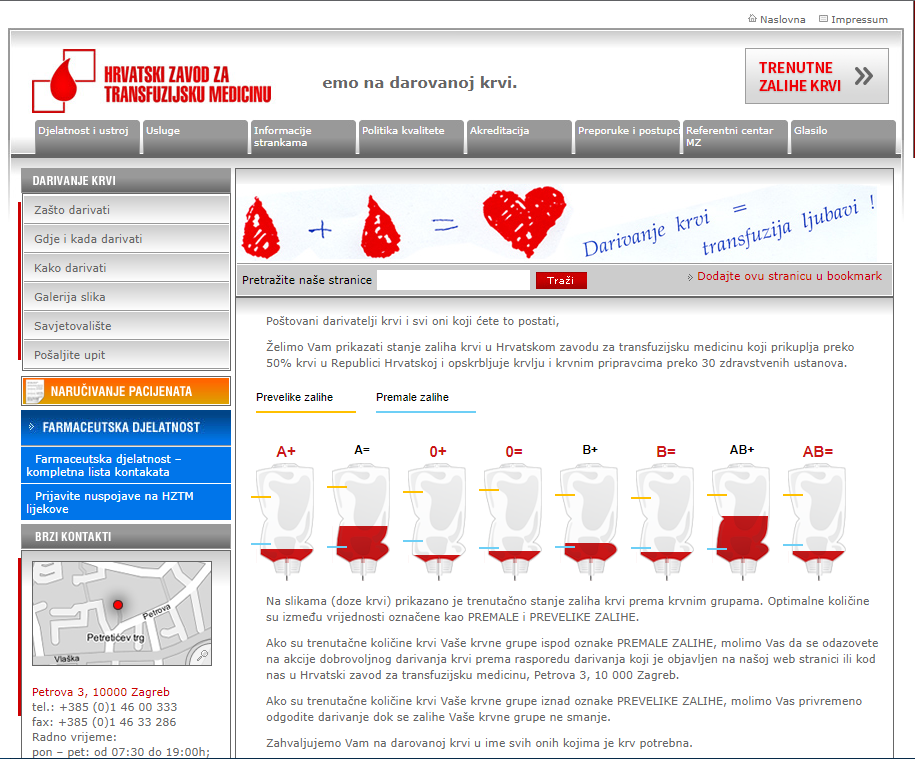
\includegraphics[scale=0.8]{slike/HZTMprimjer.PNG} %veličina slike u odnosu na originalnu datoteku i pozicija slike
			\centering
			\caption{Primjer javno dostupnih podataka o stanju banke krvi Hrvatskog zavoda za transfuzijsku medicinu}
			\label{fig:HZTMprimjer}
		\end{figure}
		\begin{figure}[H]
			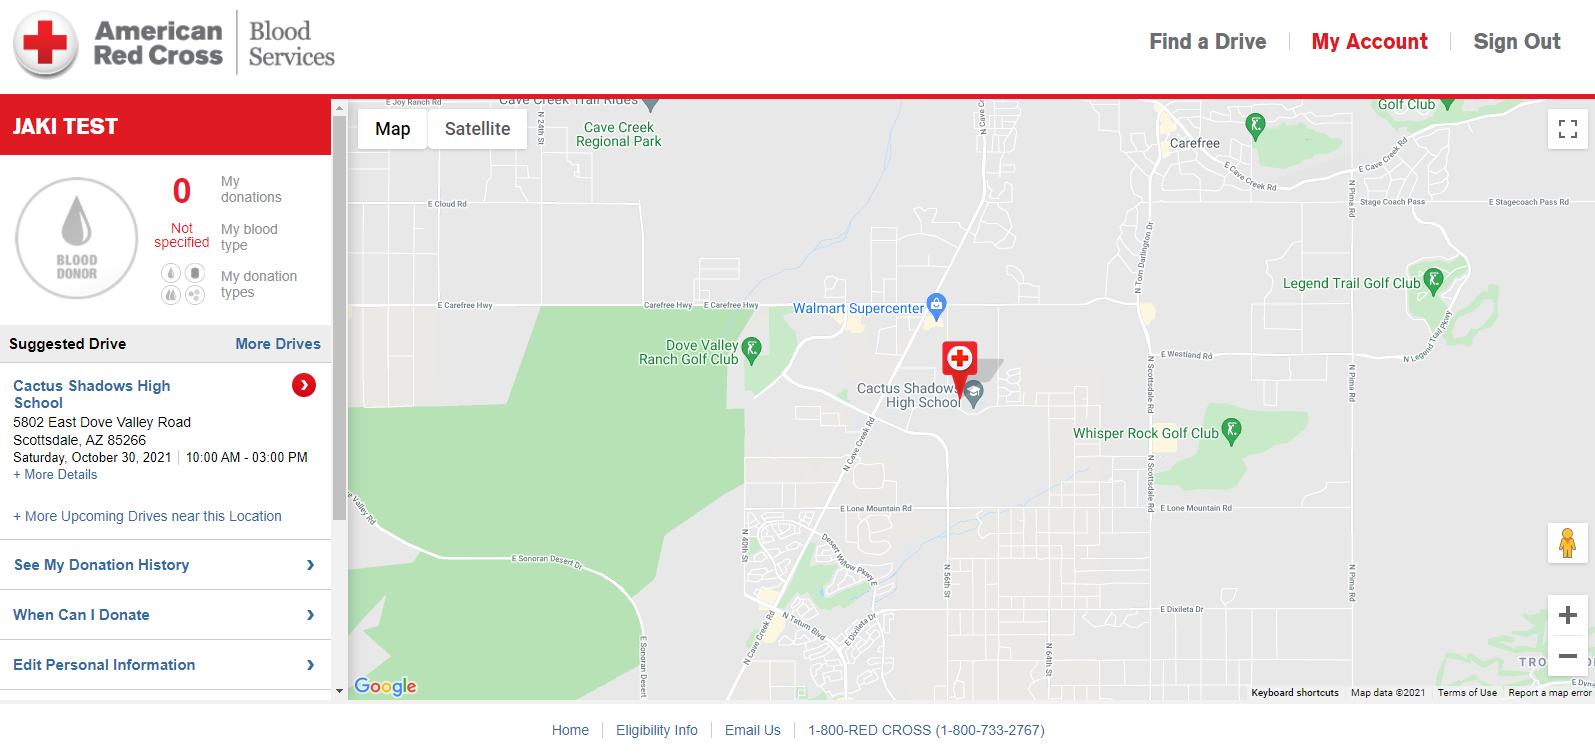
\includegraphics[scale=0.5]{slike/AmericanRedCrossPrimjer.PNG} %veličina slike u odnosu na originalnu datoteku i pozicija slike
			\centering
			\caption{Primjer web sučelja logiranog korisnika Američkog crvenog križa}
			\label{fig:AmericanRedCrossPrimjer}
		\end{figure}
		Ovo rješenje ima i nešto mjesta za kasniju nadogradnju. Jedna od mogućnosti je ugradnja podrške za notifikacije putem SMS poruka. Moguće je kasnije dodavanje i nešto poput nagradnog sistema za donore gdje bi donori svakim darivanjem krvi skupljali bodove koje bi mogli iskoristiti npr. za neke popuste kod nekih sponzora, besplatan ručak, ulaznicu u kino itd. 
		Naravno, kasnijih nadogradnji (i samih prilagodbi) može biti još, ovisno o željama i kasnijim potrebama korisnika rješenja, ukoliko su izvediva u sklopu ovog projekta.
		\eject

	
\chapter{Specifikacija programske potpore}

\section{Funkcionalni zahtjevi}

\noindent \textbf{Dionici:}

\begin{packed_enum}
	
	\item Donor		
	\item Djelatnik banke	
	\item Administrator
	\item Razvojni tim
	
\end{packed_enum}

\noindent \textbf{Aktori i njihovi funkcionalni zahtjevi:}


\begin{packed_enum}
	\item  \underbar{Neregistrirani/neprijavljeni korisnik(inicijator) može:}
	
	\begin{packed_enum}
		
		\item pregledati trenutno stanje zaliha
		\item se registrirati u sustav, stvoriti korisnički račun za koji su mu potrebni matični i kontakt podaci
		
	\end{packed_enum}
	
	\item  \underbar{Donor (inicijator) može:}
	
	\begin{packed_enum}
		
		\item pregledavati i mijenjati osobne podatke
		\item pregledavati povijest svojih doniranja
		\item iz aplikacije dobiti PDF potvrdu
		\item pregledati poruku u ovisnosti o trenutnom stanju zaliha krvi
		
	\end{packed_enum}
	
	\item  \underbar{Djelatnik banke (inicijator) može:}
	
	\begin{packed_enum}
		
		\item kreirati korisnički profil donora
		\item evidentirati svaki pokušaj doniranja (uspješan / neuspješan) 
		\item evidentirati privremeno ili trajno odbijanje
		\item evidentirati potrošnju krvi 
		\item aktivirati račun aktivacijskim linkom i odabrati lozinku
		\item vidjeti popis registriranih donora
		
	\end{packed_enum}
	\eject
	
	\item  \underbar{Administrator (inicijator) može:}
	
	\begin{packed_enum}
		
		\item definirati gornju i donju granicu optimalne količine krvi
		\item kreirati nove korisničke račune za ulogu djelatnika banke
		\item deaktivirati korisnički račun djelatnika banke ili donora
		\item vidjeti popis registriranih svih korisnika i njihovih osobnih podataka
		
	\end{packed_enum}
	
	\item  \underbar{Baza podataka (sudionik):}
	
	\begin{packed_enum}
		
		\item pohranjuje sve podatke o korisnicima i njihovim ovlastima
		\item pohranjuje trenutno stanje količine krvi,te donju i gornju granicu optimalne količine krvi
		
	\end{packed_enum}
	
	\item  \underbar{Sustav za automatske poslove(inicijator) može:}
	
	\begin{packed_enum}
		
		\item slati email notifikacije donoru nakon 3 mjeseca od uspješnog darivanja ako je muškarac ili nakon 4 mjeseca ako je žensko
		\item slati email notifikacije donoru i djelatniku banke ako se pređu granice određene krve grupe
		
	\end{packed_enum}
\end{packed_enum}



\eject 



\subsection{Obrasci uporabe}

\subsubsection{Opis obrazaca uporabe}


\noindent \underbar{\textbf{UC1 - Pregled količine krvi}}
					\begin{packed_item}
	
						\item \textbf{Glavni sudionik: }Korisnik, Donor, Djelatnik banke, Administrator
						\item \textbf{Cilj:} Prikazati trenutnu količinu krvi u banci
						\item \textbf{Sudionici:} Baza podataka
						\item \textbf{Preduvjet:} -
						\item \textbf{Opis osnovnog tijeka:}
						
						\item[] \begin{packed_enum}
	
							\item Količine krvi su prikazane otvaranjem aplikacije, te njihove gornje i donje granice
							
						\end{packed_enum}

					\end{packed_item}

\noindent \underbar{\textbf{UC2 - Registracija}}
					\begin{packed_item}
	
						\item \textbf{Glavni sudionik: }Korisnik, djelatnik banke
						\item \textbf{Cilj:} Stvoriti korisnički račun donora za pristup sustavu
						\item \textbf{Sudionici:} Baza podataka
						\item \textbf{Preduvjet:} -
						\item \textbf{Opis osnovnog tijeka:}
						
						\item[] \begin{packed_enum}
	
							\item Korisnik/Djelatnik banke odabire opciju za registraciju novog donora
							\item Korisnik/Djelatnik banke unosi potrebne podatke
							\item Korisnik/Donor na svoj mail dobiva aktivacijski link
							
						\end{packed_enum}
						
						\item  \textbf{Opis mogućih odstupanja:}
						
						\item[] \begin{packed_item}
	
							\item[2.a] Odabir već korištenog e-maila, unos podataka u nedozvoljenom formatu ili unos neispravnog e-maila
							\item[] \begin{packed_enum}
								
								\item Korisnik dobiva obavijest o neuspjelom upisu i vraća ga na stranicu za registraciju
								\item Korisnik mijenja potrebne podatke ili odustaje od registracije
								
							\end{packed_enum}
							
							
						\end{packed_item}
					\end{packed_item}
\eject 
\noindent \underbar{\textbf{UC3 - Prijava u sustav}}
					\begin{packed_item}
	
						\item \textbf{Glavni sudionik: }Donor, djelatnik
						\item \textbf{Cilj:} Prijava u sustav i dobivanje dodatnih mogućnosti aplikacije
						\item \textbf{Sudionici:} Baza podataka
						\item \textbf{Preduvjet:} Registracija
						\item \textbf{Opis osnovnog tijeka:}
						
						\item[] \begin{packed_enum}
	
							\item Unos e-maila i lozinke
							\item Potvrda ispravnosti unesenih podataka
							\item Pristup dodatnim mogućnostima
							
						\end{packed_enum}
						\item  \textbf{Opis mogućih odstupanja:}
						
						\item[] \begin{packed_item}
	
							\item[2.a] Neispravan e-mail i/ili lozinka
							\item[] \begin{packed_enum}
								
								\item  Sustav obavještava korisnika o neuspjeloj prijavi i vraća ga na stranicu za prijavu

								
							\end{packed_enum}
					\end{packed_item}
					\end{packed_item}
\noindent \underbar{\textbf{UC4 - Pregled osobnih podataka}}
					\begin{packed_item}
	
						\item \textbf{Glavni sudionik: }Donor
						\item \textbf{Cilj:} Prikazati osobne podatke prijavljenog donora
						\item \textbf{Sudionici:} Baza podataka
						\item \textbf{Preduvjet:} Donor je prijavljen
						\item \textbf{Opis osnovnog tijeka:}
						
						\item[] \begin{packed_enum}
	
							\item Donor odabire opciju "Osobni podaci"
							\item Aplikacija prikazuje osobne podatke donora
							
						\end{packed_enum}

					\end{packed_item}
\eject 
\noindent \underbar{\textbf{UC5 - Promjena matičnih i/ili kontakt podataka}}
					\begin{packed_item}
	
						\item \textbf{Glavni sudionik: }Donor
						\item \textbf{Cilj:} Promjeniti matične i/ili kotakt podatke
						\item \textbf{Sudionici:} Baza podataka
						\item \textbf{Preduvjet:} Donor je prijavljen
						\item \textbf{Opis osnovnog tijeka:}
						
						\item[] \begin{packed_enum}
	
							\item Donor odabire opciju "Promijeni osobne podatka"
							\item Donor mijenja svoje podatke
							\item Donor sprema promjene
							\item Ažurira se baza podataka
							
						\end{packed_enum}

						\item  \textbf{Opis mogućih odstupanja:}
						
						\item[] \begin{packed_item}
	
							\item[2.a] Korisnik ne spremi promjenu
							\item[] \begin{packed_enum}
								
								\item  Sustav obavještava korisnika da nije spremio podatke prilikom izlaska iz prozora

								
									\end{packed_enum}
								\end{packed_item}
					\end{packed_item}
\noindent \underbar{\textbf{UC6 - Pregled povijesti darivanja}}
					\begin{packed_item}
	
						\item \textbf{Glavni sudionik: }Donor
						\item \textbf{Cilj:} Pregledati svoju povijest darivanja krvi
						\item \textbf{Sudionici:} Baza podataka
						\item \textbf{Preduvjet:} Donor je prijavljen
						\item \textbf{Opis osnovnog tijeka:}
						
						\item[] \begin{packed_enum}
	
							\item Donor odabire opciju "Povijest darivanja"
							\item aplikacija prikazuje donorovu povijest darivanja
							
						\end{packed_enum}

					\end{packed_item}
\eject 
\noindent \underbar{\textbf{UC7 - Dobivanje PDF potvrde o doniranju}}
					\begin{packed_item}
	
						\item \textbf{Glavni sudionik: }Donor
						\item \textbf{Cilj:} Dobiti PDF potvrdu o doniranju
						\item \textbf{Sudionici:} Baza podataka
						\item \textbf{Preduvjet:} Donor je prijavljen i barem jedanput uspješno darovao krv
						\item \textbf{Opis osnovnog tijeka:}
						
						\item[] \begin{packed_enum}
	
							\item Donor odabire opciju "Povijest darivanja"
							\item Donor odabire opciju "Želim PDF potvrdu"
							\item Sustav donoru šalje potvrdu na mail
							
						\end{packed_enum}

					\end{packed_item}

\noindent \underbar{\textbf{UC8 - Dobivanje poruke stanja zalihe krvi}}
					\begin{packed_item}
	
						\item \textbf{Glavni sudionik: }Donor
						\item \textbf{Cilj:} dobiti poruku stanja zaliha krvi
						\item \textbf{Sudionici:} Baza podataka
						\item \textbf{Preduvjet:} Donor je prijavljen i nema trajnu zabranu darivanja krvi
						\item \textbf{Opis osnovnog tijeka:}
						
						\item[] \begin{packed_enum}
	
							\item Donor se prijavio u sustav
							\item Donor dobiva poruku o ovisnosti stanja zaliha krvi
							
						\end{packed_enum}

					\end{packed_item}


\noindent \underbar{\textbf{UC9 - Evidentiranje "potrošnje" krvi}}
					\begin{packed_item}
	
						\item \textbf{Glavni sudionik: }Djelatnik
						\item \textbf{Cilj:} slanje određenog broja jedinica krvi u vanjsku instituciju
						\item \textbf{Sudionici:} Baza podataka
						\item \textbf{Preduvjet:} Djelatnik je prijavljen
						\item \textbf{Opis osnovnog tijeka:}
						
						\item[] \begin{packed_enum}
	
							\item Djelatnik odabire krvnu grupu čiju zalihu želi evidentirati
							\item Djelatnik upisuje količinu
							\item Djelatnik šalje krv u vanjsku instituciju
						\end{packed_enum}
						\item  \textbf{Opis mogućih odstupanja:}
						
						\item[] \begin{packed_item}
	
							\item[2.a] Količina krvi iznosi 0
							\item[] \begin{packed_enum}
								
								\item  Sustav obavještava djelatnika da ne može poslati krv vanjskoj jedinici

								
							\end{packed_enum}
					\end{packed_item}
					\end{packed_item}

\eject 
\noindent \underbar{\textbf{UC10 - Pregled popisa registriranih donora}}
					\begin{packed_item}
	
						\item \textbf{Glavni sudionik: }Djelatnik
						\item \textbf{Cilj:} Prikazati popis svih registriranih donora
						\item \textbf{Sudionici:} Baza podataka
						\item \textbf{Preduvjet:} Djelatnik je prijavljen
						\item \textbf{Opis osnovnog tijeka:}
						
						\item[] \begin{packed_enum}
	
							\item Djelatnik odabire opciju "Popis donora"
							\item Sustav djelatniku prikazuje popis registriranih donora
						\end{packed_enum}

					\end{packed_item}


\noindent \underbar{\textbf{UC$11$ -{Aktivacija računa}	}}
\begin{packed_item}
	
	\item \textbf{Glavni sudionik: } {Korisnik, djelatnik banke}
	\item  \textbf{Cilj:} {Aktivirati račun}
	\item  \textbf{Sudionici:}{Baza podataka} 
	\item  \textbf{Preduvjet:}{Registracija}
	\item  \textbf{Opis osnovnog tijeka:}
	
	\item[] \begin{packed_enum}
		
		\item {Korisnika nakon klika na link u mailu vodi u aplikaciju}
		\item {Prikazuje se poruka o uspješnoj registraciji i traži se odabir lozinke} 
		\item {Korisnik odabire lozinku}
		\item {Korisnik se automatski prijavljuje}
		
	\end{packed_enum}
	
\end{packed_item}

\noindent \underbar{\textbf{UC$12$ -{Evidentiranje pokušaja doniranja}	}}
\begin{packed_item}
	
	\item \textbf{Glavni sudionik: }{Djelatnik banke}
	\item  \textbf{Cilj:} {Evidentirati pokušaj doniranja}
	\item  \textbf{Sudionici:}{Baza podataka} 
	\item  \textbf{Preduvjet:}{Registracija}
	\item  \textbf{Opis osnovnog tijeka:}
	
	\item[] \begin{packed_enum}
		
		\item {Djelatnik odabere opciju za evidentiranje pokušaja doniranja određenog donora}
		\item {Djelatnik evidentira s uspješan ili neuspješan pokušaj}
		\item {Djelatnik banke sprema promjene}
		\item {Baza podataka se ažurira, povećava se razina određene vrste krvi i zapisuje se pokušaj doniranja krvi}
		\item {Sustav šalje email poruku s PDF potvrdom}
		
	\end{packed_enum}
	
\end{packed_item}
\eject 
\noindent \underbar{\textbf{UC$13$ -{Brisanje donora}	}}
\begin{packed_item}
	
	\item \textbf{Glavni sudionik: }{Administrator}
	\item  \textbf{Cilj:} {Izbrisati kor. račun donora}
	\item  \textbf{Sudionici:}{Baza podataka}
	\item  \textbf{Preduvjet:}{Administrator prijavljen}
	\item  \textbf{Opis osnovnog tijeka:}
	
	\item[] \begin{packed_enum}
		
		\item {Administrator odabire opciju Prikaz donora}
		\item {Administratoru se pokažu registrirani donori} 
		\item {Administrator briše donora}
		
	\end{packed_enum}
	
\end{packed_item}

\noindent \underbar{\textbf{UC$14$ -{Definiranje optimalnih granica}	}}
\begin{packed_item}
	
	\item \textbf{Glavni sudionik: }{Administrator}
	\item  \textbf{Cilj:} {Definirati gornju i donju granicu optimalnih količina krvi za pojedinu grupu}
	\item  \textbf{Sudionici:}{Baza podataka}
	\item  \textbf{Preduvjet:}{Administrator je prijavljen}
	\item  \textbf{Opis osnovnog tijeka:}
	
	\item[] \begin{packed_enum}
		
		\item {Administrator odabire opciju "Definiraj granice"}
		\item {Prikazuju se trenutno određene granice za pojedinu vrstu krvi} 
		\item {Administrator definira granice za pojedinu vrstu krvi}
		\item {Administrator sprema promjene}
		
	\end{packed_enum}
\end{packed_item}

\noindent \underbar{\textbf{UC$15$ -{Pregled popisa djelatnika}	}}
\begin{packed_item}
	
	\item \textbf{Glavni sudionik: }{Administartor}
	\item  \textbf{Cilj:} {Prikazati popis svih djelatnika banke}
	\item  \textbf{Sudionici:}{Baza podataka} 
	\item  \textbf{Preduvjet:}{Administrator je prijavljen}
	\item  \textbf{Opis osnovnog tijeka:}
	
	\item[] \begin{packed_enum}
		
		\item {Administrator odabire opciju "Prikaz popisa djelatnika banke"}
		\item {Prikazuje se popis svih djelatnika banke po abecednom redu}
		\end{packed_enum}
\end{packed_item}

\eject 
\noindent \underbar{\textbf{UC$16$ -{Brisanje djelatnika banke}	}}
\begin{packed_item}
	
	\item \textbf{Glavni sudionik: }{Administrator}
	\item  \textbf{Cilj:} {Izbrisati kor. račun djelatnika banke}
	\item  \textbf{Sudionici:}{Baza podataka}
	\item  \textbf{Preduvjet:}{Administrator prijavljen}
	\item  \textbf{Opis osnovnog tijeka:}
	
	\item[] \begin{packed_enum}
		
		\item {Administrator odabire opciju Prikaz djelatnika banke}
		\item {Administratoru se pokažu registrirani djelatnici banke}
		\item {Administrator briše djelatnika banke}
		
	\end{packed_enum}
	
\end{packed_item}

\noindent \underbar{\textbf{UC$17$ -{Kreiranje kor. računa djelatnika banke}	}}
\begin{packed_item}
	
	\item \textbf{Glavni sudionik: }{Administrator}
	\item  \textbf{Cilj:} {Kreirati računa djelatnika banke}
	\item  \textbf{Sudionici:}{Baza podataka}
	\item  \textbf{Preduvjet:}{Administrator je prijavljen}
	\item  \textbf{Opis osnovnog tijeka:}
	
	\item[] \begin{packed_enum}
		
		\item {Administrator odabire opciju "Kreiraj korisnički račun djelatnika banke"}
		\item {Prikazuje se forma koju popunjava} 
		\item {Odabire opciju "Kreiraj račun"}
		\item {Baza podataka se ažurira}
		\item {Šalje se aktivacijski link na email djelatnika banke}
	\end{packed_enum}
	
	\item  \textbf{Opis mogućih odstupanja:}
	
	\item[] \begin{packed_item}
		
		\item[2.a] $<$opis mogućeg scenarija odstupanja u koraku 2$>$
		\item[] \begin{packed_enum}
			
			\item $<$opis rješenja mogućeg scenarija korak 1$>$
			\item $<$opis rješenja mogućeg scenarija korak 2$>$
			
		\end{packed_enum}
		\item[2.b] $<$opis mogućeg scenarija odstupanja u koraku 2$>$
		\item[3.a] $<$opis mogućeg scenarija odstupanja  u koraku 3$>$
		
	\end{packed_item}
\end{packed_item}
\eject 
\noindent \underbar{\textbf{UC$18$ -{Slanje notifikacije nakon 3/4 mjeseca}	}}
\begin{packed_item}
	
	\item \textbf{Glavni sudionik: }{Sustav za automatske poslove}
	\item  \textbf{Cilj:} {Poslati notifikaciju donoru}
	\item  \textbf{Sudionici:}{Baza podataka}
	\item  \textbf{Preduvjet:}{Prošlo 3 mjeseca od uspješnog darivanja}
	\item  \textbf{Opis osnovnog tijeka:}
	
	\item[] \begin{packed_enum}
		
		\item {Sustav svakodnevno provjerava uspješna doniranja od prije 3 mjeseca za muškarce i od prije 4 mjeseca za žene}
		\item {Svima koji zadovoljavaju uvjet šalju se email notifikacije da mogu doći ponovno donirati krv}
		
	\end{packed_enum}
	
\end{packed_item}

\noindent \underbar{\textbf{UC$19$ -{Slanje notifikacije ako se prijeđu granice}	}}
\begin{packed_item}
	
	\item \textbf{Glavni sudionik: }{Sustav za automatske poslove}
	\item  \textbf{Cilj:} {Poslati notifikaciju donoru i djelatniku banke}
	\item  \textbf{Sudionici:}{Baza podataka}
	\item  \textbf{Preduvjet:}{Prešle su se optimalne granice}
	\item  \textbf{Opis osnovnog tijeka:}
	
	\item[] \begin{packed_enum}
		
		\item {Ako je došlo do prekoračenja gornje granice šalje se notifikacija na email djelatnika banke}
		\item {Ako je došlo do pada ispod donje granice šalje se notifikacija na email donora ako je te krvne grupe i djelatniku banke}
		
		
	\end{packed_enum}
	
\end{packed_item}

\subsubsection{Dijagrami obrazaca uporabe}
\begin{figure}[H]
			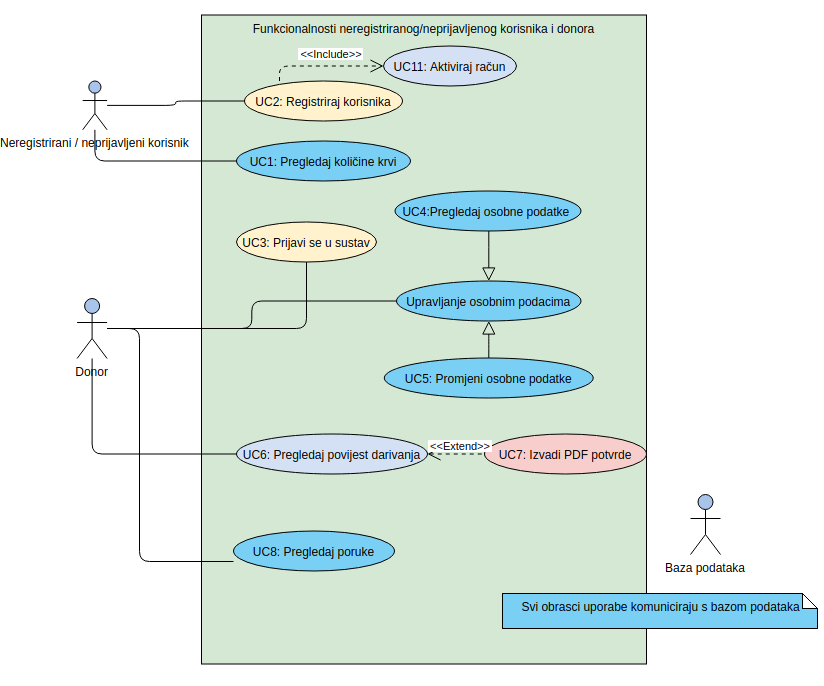
\includegraphics[scale=0.6]{dijagrami/Funkcionalnosti_korisnika_donora.png} %veličina slike u odnosu na originalnu datoteku i pozicija slike
			\centering
			\caption{Dijagram obrasca uporabe, funkcionalnost korisnika i donora}
			\label{fig:Funkcionalnosti_korisnika_donora}
\end{figure}

\begin{figure}[H]
			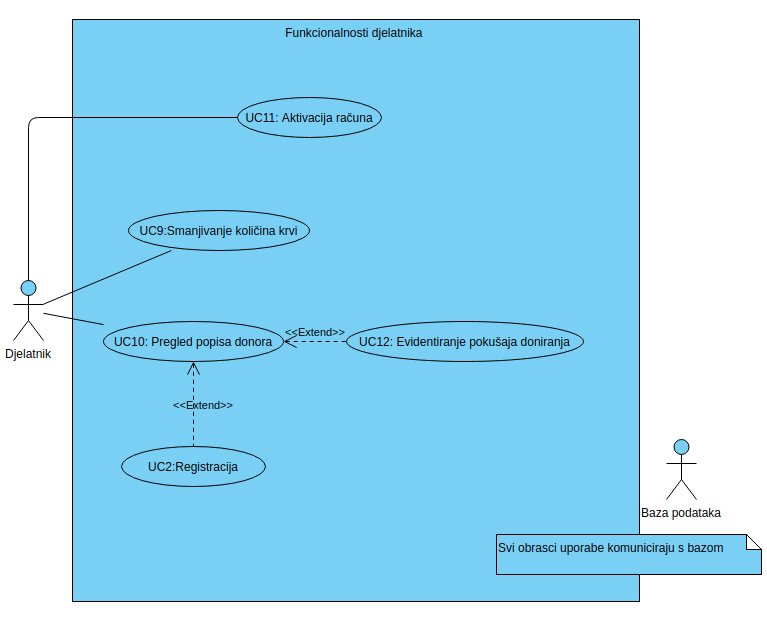
\includegraphics[scale=0.6]{dijagrami/Funkcionalnosti_djelatnika_donora.png} %veličina slike u odnosu na originalnu datoteku i pozicija slike
			\centering
			\caption{Dijagram obrasca uporabe, funkcionalnost djelatnika i donora}
			\label{fig:Funkcionalnosti_djelatnika_donora}
\end{figure}

\begin{figure}[H]
			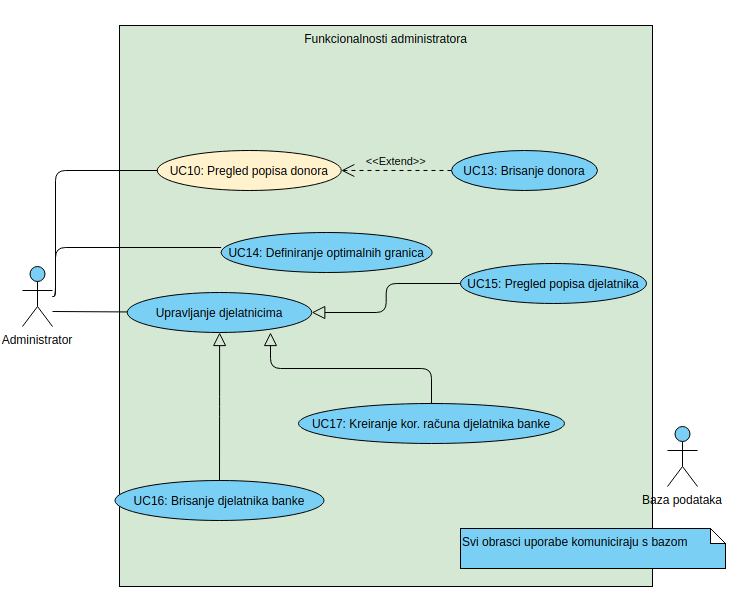
\includegraphics[scale=0.6]{dijagrami/Funkcionalnosti_admina.png} %veličina slike u odnosu na originalnu datoteku i pozicija slike
			\centering
			\caption{Dijagram obrasca uporabe, funkcionalnost administratora}
			\label{fig:Funkcionalnosti_admina}
\end{figure}

\begin{figure}[H]
			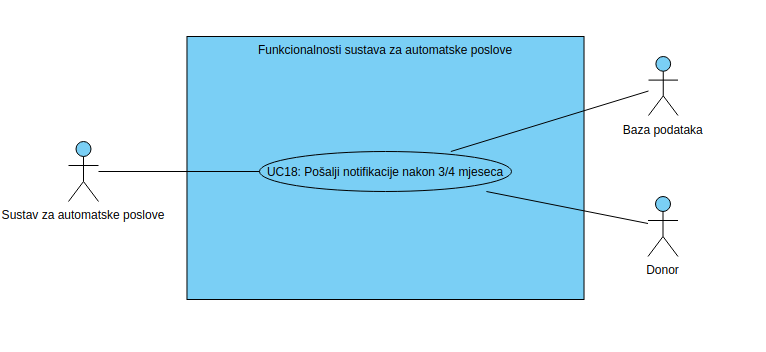
\includegraphics[scale=0.6]{dijagrami/Funkcionalnosti_auto.png} %veličina slike u odnosu na originalnu datoteku i pozicija slike
			\centering
			\caption{Dijagram obrasca uporabe, funkcionalnost sustava za automatske poslove}
			\label{fig:Funkcionalnosti_auto}
\end{figure}

\eject
		
\subsection{Sekvencijski dijagrami}

\textbf{Obrazac uporabe UC8 - Dobivanje poruke stanja zalihe krvi}

Donor, koji nema trajnu zabranu darivanja krvi, kod svakog spajanja u sustav dobiva poruku u ovisnosti o trenutnom stanju zaliha krvi. Poslužitelj dohvaća podatke iz baze podataka i prema zadanim granicama vraća jednu od tri poruka. Poruke mogu biti: stanje zaliha ispod optimalne granice; stanje zaliha je optimalno; stanje zaliha je iznad gornje optimalne granice.

\begin{figure}[H]
	\centering
	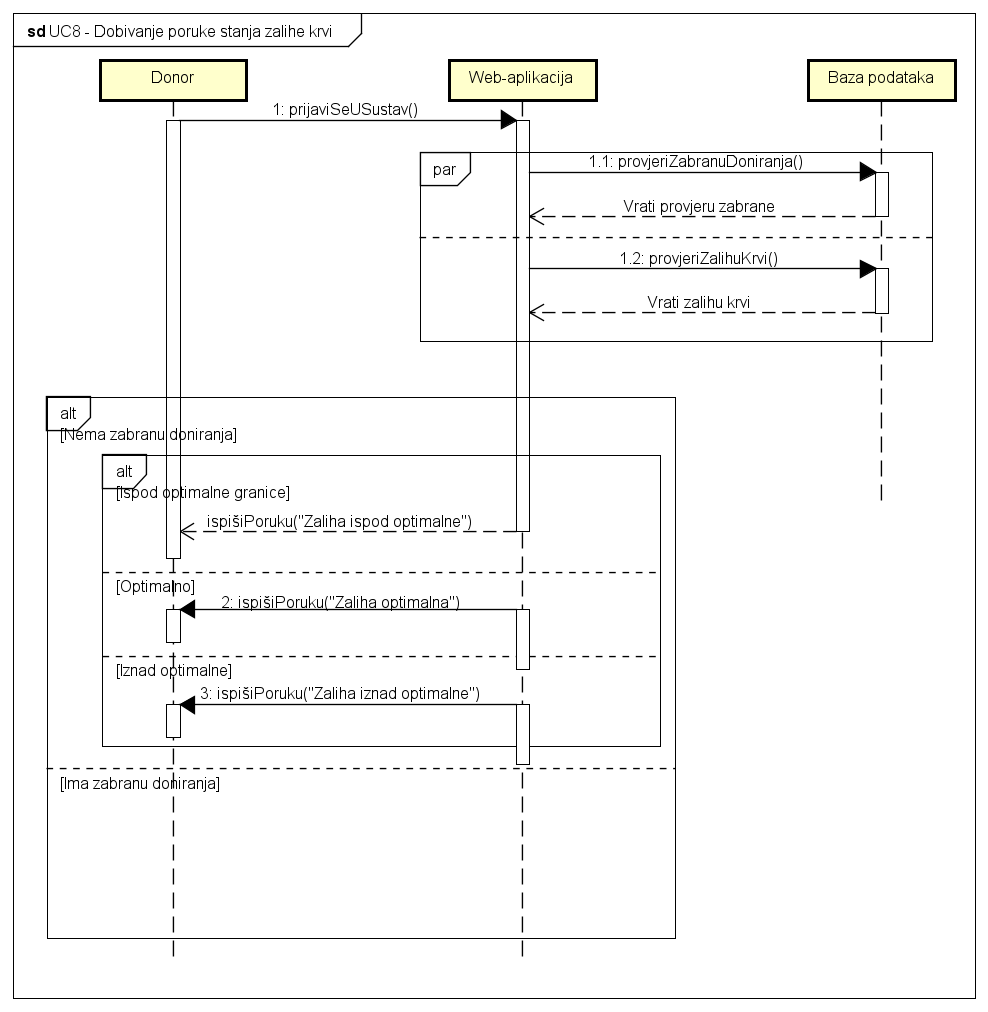
\includegraphics[width=\textwidth, scale=0.4]{dijagrami/UC8_Dobivanje poruke stanja zalihe krvi.png}
	\caption{Sekvencijski dijagram za UC8}
	\label{fig:UC8_Dobivanje poruke stanja zalihe krvi}
\end{figure}
\eject

\textbf{Obrazac uporabe UC9 - Evidentiranje "potrošnje" krvi}

Djelatnik banke može evidentirati "potrošnju" krvi odnosno slanje određenog broja jedinica krvi u vanjsku instituciju. U bazi podataka se smanjuje količina određene vrste krvi.

\begin{figure}[H]
	\centering
	\includegraphics[width=\textwidth, scale=0.4]{dijagrami/UC9_Evidentiranje_potrošnje_ krvi.png}
	\caption{Sekvencijski dijagram za UC9}
\end{figure}

\eject 
\textbf{Obrazac uporabe UC12 - Evidentiranje pokušaja doniranja}

Djelatnik banke evidentira i uspješne i neuspješne pokušaje doniranja. Na temelju zdravstvenog stanja donor može pristupiti doniranju, ali može i biti privremeno ili trajno odbijen. Baza podataka se ažurira, zapisuje se pokušaj doniranja krvi i ako je uspješan poveća se razina određene vrste krvi.

\begin{figure}[H]
	\centering
	\includegraphics[width=\textwidth]{dijagrami/UC12_Evidentiranje pokušaja doniranja.png}
	\caption{Sekvencijski dijagram za UC12}
\end{figure}
\eject

\textbf{Obrazac uporabe UC14 - Definiranje optimalnih granica}

Za svaku krvnu grupu administrator sustava definira gornju i donju granicu optimalne količine. Administratoru se prikazuju trenutne granice za pojedinu vrstu krvi. Zatim on ih on može mijenjati i promjene se spremaju i bazu podataka.

\begin{figure}[H]
	\centering
	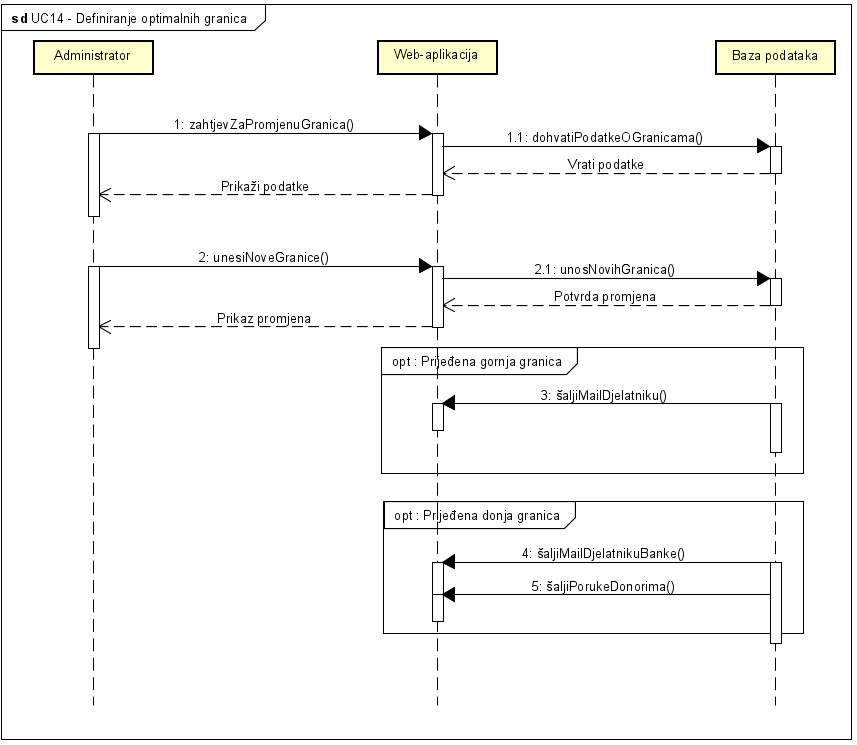
\includegraphics[width=\textwidth]{dijagrami/UC14_Definiranje optimalnih granica.png}
	\caption{Sekvencijski dijagram za UC14}
\end{figure}
\eject

\section{Ostali zahtjevi}

\textbf{\textit{dio 1. revizije}}\\

\textit{Nefunkcionalni zahtjevi i zahtjevi domene primjene dopunjuju funkcionalne zahtjeve. Oni opisuju \textbf{kako se sustav treba ponašati} i koja \textbf{ograničenja} treba poštivati (performanse, korisničko iskustvo, pouzdanost, standardi kvalitete, sigurnost...). Primjeri takvih zahtjeva u Vašem projektu mogu biti: podržani jezici korisničkog sučelja, vrijeme odziva, najveći mogući podržani broj korisnika, podržane web/mobilne platforme, razina zaštite (protokoli komunikacije, kriptiranje...)... Svaki takav zahtjev potrebno je navesti u jednoj ili dvije rečenice.}






	\chapter{Arhitektura i dizajn sustava}
		
		\textbf{\textit{dio 1. revizije}}\\

		\textit{ Potrebno je opisati stil arhitekture te identificirati: podsustave, preslikavanje na radnu platformu, spremišta podataka, mrežne protokole, globalni upravljački tok i sklopovsko-programske zahtjeve. Po točkama razraditi i popratiti odgovarajućim skicama:}
	\begin{itemize}
		\item 	\textit{izbor arhitekture temeljem principa oblikovanja pokazanih na predavanjima (objasniti zašto ste baš odabrali takvu arhitekturu)}
		\item 	\textit{organizaciju sustava s najviše razine apstrakcije (npr. klijent-poslužitelj, baza podataka, datotečni sustav, grafičko sučelje)}
		\item 	\textit{organizaciju aplikacije (npr. slojevi frontend i backend, MVC arhitektura) }		
	\end{itemize}

	
		

		

				
		\section{Baza podataka}
			
			\textbf{\textit{dio 1. revizije}}\\
			
		\textit{Potrebno je opisati koju vrstu i implementaciju baze podataka ste odabrali, glavne komponente od kojih se sastoji i slično.}
		
			\subsection{Opis tablica}
			

				\textit{Svaku tablicu je potrebno opisati po zadanom predlošku. Lijevo se nalazi točno ime varijable u bazi podataka, u sredini se nalazi tip podataka, a desno se nalazi opis varijable. Svjetlozelenom bojom označite primarni ključ. Svjetlo plavom označite strani ključ}
				
				
				\begin{longtblr}[
					label=none,
					entry=none
					]{
						width = \textwidth,
						colspec={|X[6,l]|X[6, l]|X[20, l]|}, 
						rowhead = 1,
					} %definicija širine tablice, širine stupaca, poravnanje i broja redaka naslova tablice
					\hline \multicolumn{3}{|c|}{\textbf{korisnik - ime tablice}}	 \\ \hline[3pt]
					\SetCell{LightGreen}IDKorisnik & INT	&  	Lorem ipsum dolor sit amet, consectetur adipiscing elit, sed do eiusmod  	\\ \hline
					korisnickoIme	& VARCHAR &   	\\ \hline 
					email & VARCHAR &   \\ \hline 
					ime & VARCHAR	&  		\\ \hline 
					\SetCell{LightBlue} primjer	& VARCHAR &   	\\ \hline 
				\end{longtblr}
				
				
			
			\subsection{Dijagram baze podataka}
				\textit{ U ovom potpoglavlju potrebno je umetnuti dijagram baze podataka. Primarni i strani ključevi moraju biti označeni, a tablice povezane. Bazu podataka je potrebno normalizirati. Podsjetite se kolegija "Baze podataka".}
			
			\eject
			
			
		\section{Dijagram razreda}
		
			\textit{Potrebno je priložiti dijagram razreda s pripadajućim opisom. Zbog preglednosti je moguće dijagram razlomiti na više njih, ali moraju biti grupirani prema sličnim razinama apstrakcije i srodnim funkcionalnostima.}\\
			
			\textbf{\textit{dio 1. revizije}}\\
			
			\textit{Prilikom prve predaje projekta, potrebno je priložiti potpuno razrađen dijagram razreda vezan uz \textbf{generičku funkcionalnost} sustava. Ostale funkcionalnosti trebaju biti idejno razrađene u dijagramu sa sljedećim komponentama: nazivi razreda, nazivi metoda i vrste pristupa metodama (npr. javni, zaštićeni), nazivi atributa razreda, veze i odnosi između razreda.}\\
			
			\textbf{\textit{dio 2. revizije}}\\			
			
			\textit{Prilikom druge predaje projekta dijagram razreda i opisi moraju odgovarati stvarnom stanju implementacije}
			
			
			
			\eject
		
		\section{Dijagram stanja}
			
			
			\textbf{\textit{dio 2. revizije}}\\
			
			\textit{Potrebno je priložiti dijagram stanja i opisati ga. Dovoljan je jedan dijagram stanja koji prikazuje \textbf{značajan dio funkcionalnosti} sustava. Na primjer, stanja korisničkog sučelja i tijek korištenja neke ključne funkcionalnosti jesu značajan dio sustava, a registracija i prijava nisu. }
			
			
			\eject 
		
		\section{Dijagram aktivnosti}
			
			\textbf{\textit{dio 2. revizije}}\\
			
			 \textit{Potrebno je priložiti dijagram aktivnosti s pripadajućim opisom. Dijagram aktivnosti treba prikazivati značajan dio sustava.}
			
			\eject
		\section{Dijagram komponenti}
		
			\textbf{\textit{dio 2. revizije}}\\
		
			 \textit{Potrebno je priložiti dijagram komponenti s pripadajućim opisom. Dijagram komponenti treba prikazivati strukturu cijele aplikacije.}
	\chapter{Implementacija i korisničko sučelje}
		
		
		\section{Korištene tehnologije i alati}
		
			\textbf{\textit{dio 2. revizije}}
			
			 \textit{Detaljno navesti sve tehnologije i alate koji su primijenjeni pri izradi dokumentacije i aplikacije. Ukratko ih opisati, te navesti njihovo značenje i mjesto primjene. Za svaki navedeni alat i tehnologiju je potrebno \textbf{navesti internet poveznicu} gdje se mogu preuzeti ili više saznati o njima}.
			
			
			\eject 
		
	
		\section{Ispitivanje programskog rješenja}
			
Nakon što smo završili s izradom testirali smo rad aplikacije koristeći JUnit tehnologiju i
Selenium WebDriver. Testovi su dali zadovoljavajuće rezultate te možemo zaključiti da smo uspjeli implementirati zadane funkcionalnosti.
			
			\subsection{Ispitivanje komponenti}
			
Za ispitivanje komponenti koristili smo JUnit tehnologiju. JUnit okvir je za testiranje komponenti sustava programiranog u Javi. Ispitali smo funkcionalnosti ažuriranja osobnih podataka donora, promjenu optimalnih granica krvi i evidencije krvi slanjem u instituciju. Koriste se objekti tipa UserContoller, BloodController i ConsumptionController na kojima se pozivaju ispitivane funkcionalnosti te UserService, BloodService i RoleService koji su potrebni za dohvaćanje podataka korištenih u funkcijama.
\\\\
\textbf{Ažuriranje osobnih podataka donora}
\\\\
Pozivom funkcije getEditUserInfo iz klase UserController želimo donoru uspješno promijeniti prezime. Na kraju uspoređujemo je li prezime ažuriranog donora jednako željenom novom prezimenu.
\\\\
\begin{figure}[H]
	\centering
	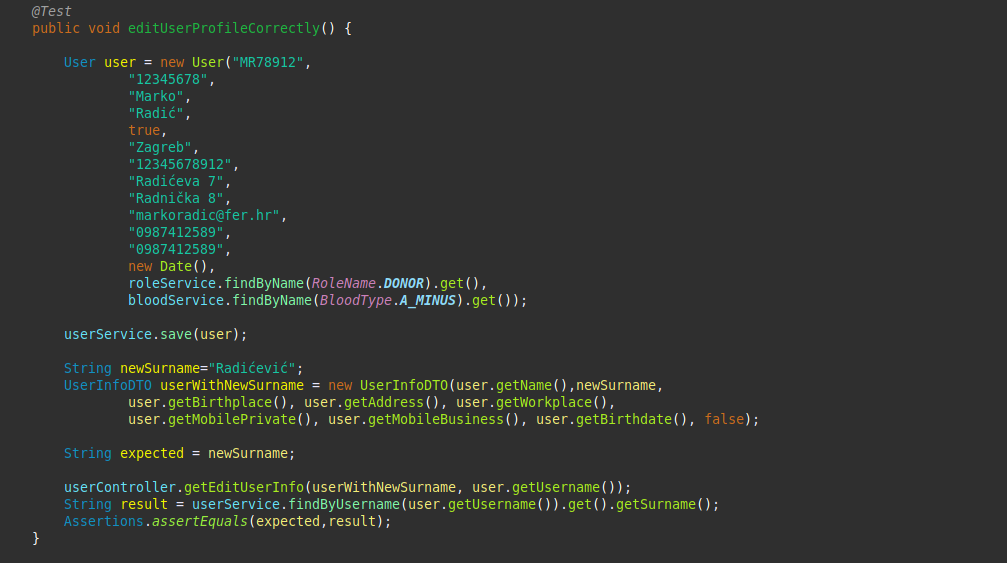
\includegraphics[width=\textwidth, scale=0.5]{dijagrami/unit1}
	\caption{Unit test1}
\end{figure}
	
U idućem testu pozivom iste funkcije želimo neuspješno ažurirati polje rejected, koje se ne bi smjelo mijenjati. Na kraju uspoređujemo je li dobivena statusn poruka jednaka očekivanoj "400" što bi značilo da aplikacija na pobuđeno situaciju prikladno odgovara.

	
			
			
			\subsection{Ispitivanje sustava}
			
			 \textit{Potrebno je provesti i opisati ispitivanje sustava koristeći radni okvir Selenium\footnote{\url{https://www.seleniumhq.org/}}. Razraditi \textbf{minimalno 4 ispitna slučaja} u kojima će se ispitati redovni slučajevi, rubni uvjeti te poziv funkcionalnosti koja nije implementirana/izaziva pogrešku kako bi se vidjelo na koji način sustav reagira kada nešto nije u potpunosti ostvareno. Ispitni slučaj se treba sastojati od ulaza (npr. korisničko ime i lozinka), očekivanog izlaza ili rezultata, koraka ispitivanja i dobivenog izlaza ili rezultata.\\ }
			 
			 \textit{Izradu ispitnih slučajeva pomoću radnog okvira Selenium moguće je provesti pomoću jednog od sljedeća dva alata:}
			 \begin{itemize}
			 	\item \textit{dodatak za preglednik \textbf{Selenium IDE} - snimanje korisnikovih akcija radi automatskog ponavljanja ispita	}
			 	\item \textit{\textbf{Selenium WebDriver} - podrška za pisanje ispita u jezicima Java, C\#, PHP koristeći posebno programsko sučelje.}
			 \end{itemize}
		 	\textit{Detalji o korištenju alata Selenium bit će prikazani na posebnom predavanju tijekom semestra.}
			
			\eject 
		
		
		\section{Dijagram razmještaja}
			
			Dijagrami razmještaja prikazuju topologiju sustava i odnos sklopovskih i program-
skih dijelova. Olakšavaju nam vizualizaciju razmještaja fizičkog dijela sustava i
sklopovlja. Sustav se sastoji od klijentskog i poslužiteljskog računala. Klijent na
svojem računalu preko web preglednika pristupa aplikaciji. Klijentsko računalo
komunicira s poslužiteljskim računalom preko HTTP veze. Na poslužiteljskom se
računalu nalaze web poslužitelj i poslužitelj baze podataka (PostgreSQL).

\begin{figure}[H]
	\centering
	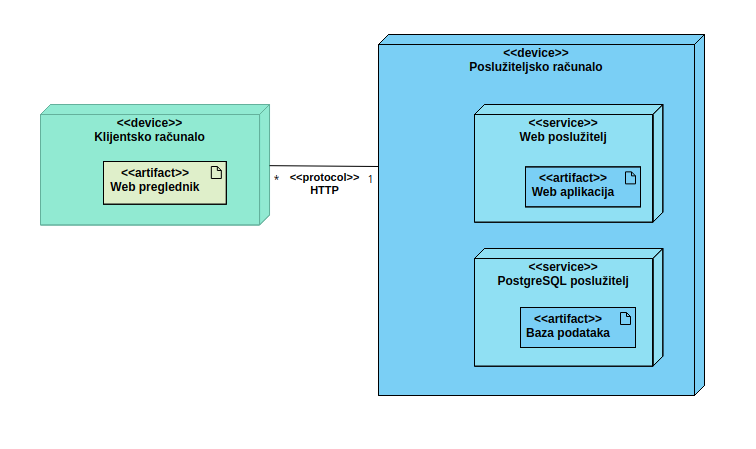
\includegraphics[width=\textwidth, scale=0.5]{dijagrami/dijagram_razmjestaja}
	\caption{Dijagram razmještaja}
	\label{fig:dijagram_razmještaja}
\end{figure}
			
			
			\eject 
		
		\section{Upute za puštanje u pogon}
		
			\textbf{\textit{dio 2. revizije}}\\
		
			 \textit{U ovom poglavlju potrebno je dati upute za puštanje u pogon (engl. deployment) ostvarene aplikacije. Na primjer, za web aplikacije, opisati postupak kojim se od izvornog kôda dolazi do potpuno postavljene baze podataka i poslužitelja koji odgovara na upite korisnika. Za mobilnu aplikaciju, postupak kojim se aplikacija izgradi, te postavi na neku od trgovina. Za stolnu (engl. desktop) aplikaciju, postupak kojim se aplikacija instalira na računalo. Ukoliko mobilne i stolne aplikacije komuniciraju s poslužiteljem i/ili bazom podataka, opisati i postupak njihovog postavljanja. Pri izradi uputa preporučuje se \textbf{naglasiti korake instalacije uporabom natuknica} te koristiti što je više moguće \textbf{slike ekrana} (engl. screenshots) kako bi upute bile jasne i jednostavne za slijediti.}
			
			
			 \textit{Dovršenu aplikaciju potrebno je pokrenuti na javno dostupnom poslužitelju. Studentima se preporuča korištenje neke od sljedećih besplatnih usluga: \href{https://aws.amazon.com/}{Amazon AWS}, \href{https://azure.microsoft.com/en-us/}{Microsoft Azure} ili \href{https://www.heroku.com/}{Heroku}. Mobilne aplikacije trebaju biti objavljene na F-Droid, Google Play ili Amazon App trgovini.}
			
			
			\eject 
	\begin{document}
	content...

\chapter{Zaključak i budući rad}
		
		\textbf{\textit{dio 2. revizije}}\\
		
		 \textit{U ovom poglavlju potrebno je napisati osvrt na vrijeme izrade projektnog zadatka, koji su tehnički izazovi prepoznati, jesu li riješeni ili kako bi mogli biti riješeni, koja su znanja stečena pri izradi projekta, koja bi znanja bila posebno potrebna za brže i kvalitetnije ostvarenje projekta i koje bi bile perspektive za nastavak rada u projektnoj grupi.}
		
		 \textit{Potrebno je točno popisati funkcionalnosti koje nisu implementirane u ostvarenoj aplikaciji.}
		
		\eject \end{document}

	\chapter*{Popis literature}
		\addcontentsline{toc}{chapter}{Popis literature}
	 	
 		\textbf{\textit{Kontinuirano osvježavanje}}
	
		\textit{Popisati sve reference i literaturu koja je pomogla pri ostvarivanju projekta.}
		
		
		\begin{enumerate}
			
			
			\item  Programsko inženjerstvo, FER ZEMRIS, \url{http://www.fer.hr/predmet/proinz}
			
			\item  I. Sommerville, "Software engineering", 8th ed, Addison Wesley, 2007.
			
			\item  T.C.Lethbridge, R.Langaniere, "Object-Oriented Software Engineering", 2nd ed. McGraw-Hill, 2005.
			
			\item  I. Marsic, Software engineering book``, Department of Electrical and Computer Engineering, Rutgers University, \url{http://www.ece.rutgers.edu/~marsic/books/SE}
			
			\item  The Unified Modeling Language, \url{https://www.uml-diagrams.org/}
			
			\item  Astah Community, \url{http://astah.net/editions/uml-new}
		\end{enumerate}
		
		 
	
	
	\begingroup
	\renewcommand*\listfigurename{Indeks slika i dijagrama}
	%\renewcommand*\listtablename{Indeks tablica}
	%\let\clearpage\relax
	\listoffigures
	%\vspace{10mm}
	%\listoftables
	\endgroup
	\addcontentsline{toc}{chapter}{Indeks slika i dijagrama}


	
	\eject 
		
	\chapter*{Dodatak: Prikaz aktivnosti grupe}
		\addcontentsline{toc}{chapter}{Dodatak: Prikaz aktivnosti grupe}
		
		\section*{Dnevnik sastajanja}
		
		
		\begin{packed_enum}
			\item  sastanak
			
			\item[] \begin{packed_item}
				\item Datum: 14. listopada 2021.
				\item Prisustvovali: Svi
				\item Teme sastanka:
				\begin{packed_item}
					\item  inicijalni dogovor s CROZ djelatnicima
				\end{packed_item}
			\end{packed_item}
			
			\item  sastanak
			\item[] \begin{packed_item}
				\item Datum: 21. listopada 2021.
				\item Prisustvovali: Svi
				\item Teme sastanka:
				\begin{packed_item}
					\item  dogovor oko podjele zadataka
					\item  podijeljeni zadaci iz dokumentacije na sedmero ljudi
				\end{packed_item}
			\end{packed_item}
			\item  sastanak
			\item[] \begin{packed_item}
				\item Datum: 28. listopada 2021.
				\item Prisustvovali: Jurinić, Kerman
				\item Teme sastanka:
				\begin{packed_item}
					\item  pripremljeni obrasci uporabe
					\item  podjela oko crtanja i opisivanja dijagrama
				\end{packed_item}
			\end{packed_item}
			\item  sastanak
			\item[] \begin{packed_item}
				\item Datum: 05. studenoga 2021.
				\item Prisustvovali: Jurinić, Hudiček, Vugrinec, Šlezak, Kerman
				\item Teme sastanka:
				\begin{packed_item}
					\item  klijentski dio aplikacije
					\item  dogovor oko poslužitelja
				\end{packed_item}
			\end{packed_item}
\eject
			\item  sastanak
			\item[] \begin{packed_item}
				\item Datum: 12. studenoga 2021.
				\item Prisustvovali: Jurinić, Hudiček, Vugrinec, Šlezak, Okreša, Kerman
				\item Teme sastanka:
				\begin{packed_item}
					\item  poslužiteljski dio aplikacije, dogovor oko dizajna baze podataka
				\end{packed_item}
			\end{packed_item}
			
			%
			
		\end{packed_enum}
		
		\eject
		\section*{Tablica aktivnosti}
		
		
			
			 \textit{Napomena: Doprinose u aktivnostima treba navesti u satima po članovima grupe po aktivnosti.}

			\begin{longtblr}[
					label=none,
				]{
					vlines,hlines,
					width = \textwidth,
					colspec={X[7, l]X[1, c]X[1, c]X[1, c]X[1, c]X[1, c]X[1, c]X[1, c]}, 
					vline{1} = {1}{text=\clap{}},
					hline{1} = {1}{text=\clap{}},
					rowhead = 1,
				} 
				\multicolumn{1}{c|}{} & \multicolumn{1}{c|}{\rotatebox{90}{\textbf{David Kerman}}} & \multicolumn{1}{c|}{\rotatebox{90}{\textbf{Ivan Jurinić}}} &	\multicolumn{1}{c|}{\rotatebox{90}{\textbf{Matija Vugrinec}}} & \multicolumn{1}{c|}{\rotatebox{90}{\textbf{Jakov Šlezak}}} &	\multicolumn{1}{c|}{\rotatebox{90}{\textbf{Matej Hudiček}}} & \multicolumn{1}{c|}{\rotatebox{90}{\textbf{Marko Okreša}}} &	\multicolumn{1}{c|}{\rotatebox{90}{\textbf{Josip Pardon}}} \\  
				Upravljanje projektom 		& 4 &  &  &  &  &  & \\ 
				Opis projektnog zadatka 	&  &  &  &  &  &  & \\ 
				
				Funkcionalni zahtjevi       & 1 & 1 &  &  &  &  &  \\ 
				Opis pojedinih obrazaca 	& 3 & 3 &  &  &  &  &  \\ 
				Dijagram obrazaca 			& 4 & 4 &  &  &  &  &  \\ 
				Sekvencijski dijagrami 		&  &  &  &  &  &  &  \\ 
				Opis ostalih zahtjeva 		&  &  &  &  &  &  &  \\ 

				Arhitektura i dizajn sustava	 & 2 &  &  &  &  &  &  \\ 
				Baza podataka				&  &  &  &  &  &  &   \\ 
				Dijagram razreda 			&  &  &  &  &  &  &   \\ 
				Dijagram stanja				&  &  &  &  &  &  &  \\ 
				Dijagram aktivnosti 		&  &  &  &  &  &  &  \\ 
				Dijagram komponenti			&  &  &  &  &  &  &  \\ 
				Korištene tehnologije i alati 		&  &  &  &  &  &  &  \\ 
				Ispitivanje programskog rješenja 	&  &  &  &  &  &  &  \\ 
				Dijagram razmještaja			&  &  &  &  &  &  &  \\ 
				Upute za puštanje u pogon 		&  &  &  &  &  &  &  \\  
				Dnevnik sastajanja 			&  &  &  &  &  &  &  \\ 
				Zaključak i budući rad 		&  &  &  &  &  &  &  \\  
				Popis literature 			&  &  &  &  &  &  &  \\  
				&  &  &  &  &  &  &  \\ \hline 
				\textit{Dodatne stavke kako ste podijelili izradu aplikacije} 			&  &  &  &  &  &  &  \\ 
				\textit{npr. izrada početne stranice} 				&  &  &  &  &  &  &  \\  
				\textit{izrada baze podataka} 		 			&  &  &  &  &  &  & \\  
				\textit{spajanje s bazom podataka} 							&  &  &  &  &  &  &  \\ 
				\textit{back end} 							&  &  &  &  &  &  &  \\  
				 							&  &  &  &  &  &  &\\ 
			\end{longtblr}
					
					
		\eject
		\section*{Dijagrami pregleda promjena}
		
		\textbf{\textit{dio 2. revizije}}\\
		
		\textit{Prenijeti dijagram pregleda promjena nad datotekama projekta. Potrebno je na kraju projekta generirane grafove s gitlaba prenijeti u ovo poglavlje dokumentacije. Dijagrami za vlastiti projekt se mogu preuzeti s gitlab.com stranice, u izborniku Repository, pritiskom na stavku Contributors.}
		
	


\end{document} %naredbe i tekst nakon ove naredbe ne ulaze u izgrađen dokument 


